\chapter{绪论}\label{chap:intro}

鲜切苹果因食用便捷、营养价值较高而受到广泛欢迎\citep{Arnold2022CRFSFS}，但切割损伤会诱发局部氧化应激与酶促褐变反应，进而导致色泽劣变、风味下降及货架期缩短\citep{Fan2023CRFSN}。围绕鲜切苹果褐变形成、护色剂作用位置以及品质保持机制开展系统研究，对于鲜切果蔬精准护色与品质调控具有重要意义。

\section{苹果XXX}\label{sec:intro-background}

鲜切苹果在加工、贮运与销售过程中易发生褐变，其本质与切割损伤后酚类底物、多酚氧化酶、氧气以及细胞结构破坏之间的耦合作用密切相关\citep{Sui2023EBC,Zeng2025FoodControl,Liu2025CRFSFS}。

\subsection{苹果XXX}\label{subsec:intro-status}

目前关于鲜切苹果褐变的研究已从整体品质评价逐步拓展到组织结构等方面。目前关于鲜切苹果褐变的研究已从整体品质评价逐步拓展到组织结构等方面。目前关于鲜切苹果褐变的研究已从整体品质评价逐步拓展到组织结构等方面。

\section{苹果XXX}\label{sec:intro-review}

现有文献多围绕抗坏血酸、柠檬酸、钙盐等护色剂的应用展开，并结合综合色差、褐变指数、酶活性变化和营养保持水平评价处理效果。现有文献多围绕抗坏血酸、柠檬酸、钙盐等护色剂的应用展开，并结合综合色差、褐变指数、酶活性变化和营养保持水平评价处理效果。

\subsection{苹果XXX}\label{subsec:intro-progress}

在褐变抑制方面，研究重点已由单纯的工艺经验优化逐渐转向机制解释。在褐变抑制方面，研究重点已由单纯的工艺经验优化逐渐转向机制解释。在褐变抑制方面，研究重点已由单纯的工艺经验优化逐渐转向机制解释。

\section{研究意义与内容}\label{sec:intro-significance-content}

本研究以鲜切苹果为对象，拟从XXX等角度，构建鲜切苹果褐变抑制与品质保持机制的研究框架。

\subsection{研究意义}\label{subsec:intro-significance}

通过明确抗坏血酸在鲜切苹果组织中的XXXX，可为鲜切果蔬护色技术的精准调控提供理论依据，并为后续开发高效护色工艺和评价体系提供参考。

\subsection{研究内容}\label{subsec:intro-contents}

研究内容主要包括：鲜切苹果褐变XXXX；外源抗坏血酸XXXX；典型处理条件下品质保持效果评价；以及基于XXXX的褐变抑制机制解析。

\section{研究路线}\label{sec:intro-route}

%本节用于放置论文技术路线图或研究思路图，后续可根据课题需要替换为正式图片。

\begin{center}
	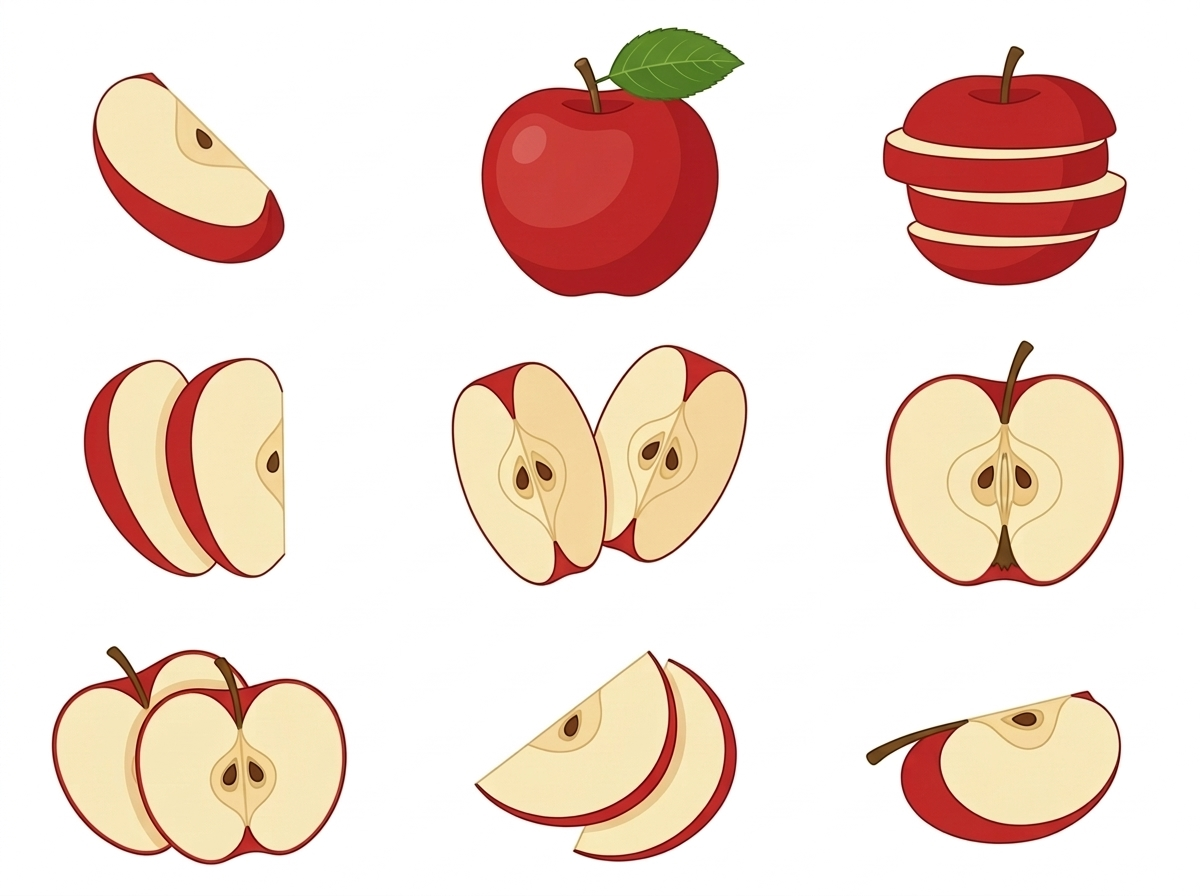
\includegraphics[width=0.6\textwidth]{figures/apple.png}
	\captionof{figure}[研究路线]{研究路线\par
		{\qauTimes\fontsize{10.5bp}{15.75bp}\selectfont \textbf{Fig.~\thefigure\ Research route}}}
	\label{fig:research-route}
\end{center}